\documentclass[11pt]{article}
\usepackage[margin=1in]{geometry}
\usepackage{times}
\renewcommand{\ttdefault}{cmtt}
\usepackage{graphicx}
\usepackage{booktabs}
\usepackage{amsmath}
\usepackage{hyperref}
\usepackage{caption}
\usepackage{subcaption}
\IfFileExists{enumitem.sty}{\usepackage{enumitem}\setlist{nosep}}{}
\captionsetup{font=small}
\title{CreditRisk Interpretation RAG System: Leakage-Aware Default-Risk Modeling for LendingClub Loans}
\author{Linda Perez Penaranda \and Yashaswi Aryan \and Siddharth Agarwal}
\date{}

\begin{document}
\sloppy
\maketitle

\begin{abstract}
This project studies default-risk prediction for accepted LendingClub loans using the Kaggle ``All Lending Club loan data'' release. The completed system is a leakage-aware tabular machine-learning pipeline, not a production lending system: it defines a binary charge-off target, excludes unresolved loans, removes post-origination leakage fields, uses chronological validation, compares major model families, calibrates probabilities, and interprets the selected model with SHAP. From 2,260,701 accepted-loan rows, the clean completed modeling frame contains 1,345,310 rows. The preferred no-grade neutral XGBoost model predicts $P(\texttt{target\_bad}=1)$ and obtains test ROC-AUC 0.710, PR-AUC 0.381, and top-20\% bad-rate concentration near 40\%. The main limitation is selection bias: repayment outcomes are observed only for accepted loans, while the future RAG adverse-action explanation layer remains planned rather than compliance-ready.
\end{abstract}

\section{Introduction}
Marketplace lending creates a natural machine-learning problem: lenders need to identify applications with elevated probability of nonpayment while avoiding broad or poorly explained denials. LendingClub's public data are useful for this task because the accepted-loan file contains borrower, loan, pricing, and credit-bureau-style variables together with eventual repayment outcomes. The primary supervised task in this project is binary classification of completed accepted loans, where \texttt{target\_bad}=0 denotes \texttt{Fully Paid} and \texttt{target\_bad}=1 denotes \texttt{Charged Off}.

The dataset is also risky to model naively. First, the bad class is a minority class, so accuracy can hide poor default detection. Second, loan vintages span changing borrower mix, underwriting rules, and macroeconomic conditions, so random splits can overstate stability. Third, many LendingClub fields are post-origination servicing or collection variables that would leak the answer if used as predictors. Rejected applications are analytically distinct: they do not contain repayment outcomes, so they cannot be labeled as default or non-default for supervised default prediction.

The non-technical solution is an auditable risk-ranking workflow. We clean application-time features, remove outcome leakage, train models on older loans, validate on later loans, reserve the newest loans for test evaluation, calibrate probabilities, and convert scores into a capped economic review policy. SHAP interpretation provides technical reasons for model behavior and is positioned as a bridge to a future RAG explanation layer, not as a legally approved adverse-action system.

\section{Proposed Method Summary}
The final method is a leakage-controlled accepted-loan default-risk pipeline using chronological train/validation/test splits, cleaned application-time features, multiple model families, calibration, SHAP interpretation, and a capped economic policy. This is preferable to simply optimizing F1 because the best-F1 threshold flags about 42\% of test loans, which is too broad for realistic underwriting review, and preferable to directly relying on LendingClub grade/subgrade because those fields embed LendingClub's prior risk decisioning. The selected neutral XGBoost model removes explicit grade and subgrade while retaining \texttt{int\_rate\_clean}, preserving nearly identical ranking performance with a simpler governance story.

\section{Related Work}
Gupta, Gulati, and Chakrabarty study the same Kaggle LendingClub dataset for credit-risk classification, using exploratory analysis, Logistic Regression, Random Forest, and expected-loss concepts such as probability of default, loss given default, and exposure at default \cite{gupta2022}. Their work motivates the connection between default prediction and financial risk, while this project adds stricter leakage documentation, chronological validation, and operating-policy constraints.

Explainability is central in recent LendingClub credit-scoring studies. Hadji Misheva et al. apply models including Logistic Regression, Random Forest, XGBoost, SVMs, and neural networks with LIME and SHAP explanations on LendingClub-style credit-risk data \cite{misheva2021}. Demajo, Vella, and Dingli similarly use XGBoost with global and local explanation methods for LendingClub and HELOC credit scoring \cite{demajo2020}. This project follows that separation between predictive modeling and explanation, but avoids presenting SHAP output as a legally compliant adverse-action explanation.

Sanz-Guerrero and Arroyo show that borrower-written loan descriptions can add risk signal through a BERT-derived indicator combined with XGBoost \cite{sanz2024}. This is relevant to the proposed RAG direction, but the current implementation intentionally avoids free-text fields because they raise privacy, proxy-risk, and applicant-facing explanation concerns. Schwartz, Wang, and Fang use SHAP-guided feature reduction and glass-box models to improve interpretability with fewer variables \cite{schwartz2025}; this supports our no-grade/subgrade ablation and the preference for a defensible feature policy over maximum complexity.

More complex work explores optimized ensembles and monitoring. Nortey et al. report strong LendingClub default-prediction results from particle-swarm tuning and greedy weighted ensembles \cite{nortey2026}. Solozobov studies label-free evidence degradation monitoring for LendingClub credit-risk systems when outcomes arrive late \cite{solozobov2026}. These papers suggest possible future improvements, but they also highlight why this class project emphasizes reproducible validation, calibration, and monitoring caveats rather than claiming production readiness.

\section{Related Implementations}
The Kaggle dataset page by Nathan George provides the accepted and rejected LendingClub files and links to getting-started notebooks for both Python and R \cite{kaggledata,kagglepython,kaggler}. Those examples focus on initial loading and EDA for a large public dataset. This project goes further by freezing a completed-loan target, documenting leakage exclusions, using chronological splits, comparing model families, and translating model scores into a capped policy.

Mariia Gusarova's Kaggle notebook focuses on outlier detection and removal using the same ``All Lending Club loan data'' input \cite{kaggleoutliers}. That style of implementation is useful for data-quality thinking, but this project avoids automatic deletion of suspicious values without documented business rules.

\section{Dataset and Inputs}
The raw source is the Kaggle ``All Lending Club loan data'' dataset, which contains separate accepted and rejected files \cite{kaggledata}. The accepted-loan file used here has 2,260,701 rows and 151 columns covering 2007--2018Q4. The rejected-application file is useful for population comparison, but rejected applicants did not receive LendingClub loans in this file, so their repayment outcomes are unobserved and they are not used as supervised default labels.

The modeling target is built from completed accepted-loan outcomes. The final strict target maps \texttt{Fully Paid} to 0 and \texttt{Charged Off} to 1. Unresolved or snapshot statuses such as \texttt{Current}, \texttt{In Grace Period}, and late-status records are excluded from final binary training because their ultimate repayment outcomes are unknown or not terminal under the strict baseline definition. After cleaning, the completed modeling frame contains 1,345,310 rows and 38 starter features.

Cleaning preserves raw fields and creates auditable helper variables. Percentage strings become numeric values such as \texttt{int\_rate\_clean} and \texttt{revol\_util\_clean}; \texttt{term} is parsed into \texttt{term\_months}; employment length is normalized; date fields are parsed; and FICO range endpoints are averaged. Clear leakage fields are removed, including payment totals, principal recovery, recoveries, collection fees, last payment dates, last credit-pull fields, hardship fields, settlement fields, and other post-origination servicing variables.

\section{Data Analysis}
EDA began with a reproducible accepted-loan working sample and full-file loan-status scans. The full file is dominated by fully paid and current loans, with charged-off loans forming the main observed bad outcome. This confirmed that current loans should not be treated as good loans: doing so would convert censored, still-active accounts into false non-default labels.

Risk relationships are strong and monotonic for several LendingClub credit variables. Grade and subgrade separate bad rates clearly, and interest rate is a dominant pricing/risk signal. Figure~\ref{fig:eda-grade} shows the observed bad-rate relationship by grade. The pattern is useful for EDA, but the final preferred model removes explicit grade and subgrade to avoid circular dependence on LendingClub's internal prior risk buckets.

\begin{figure}[h]
\centering
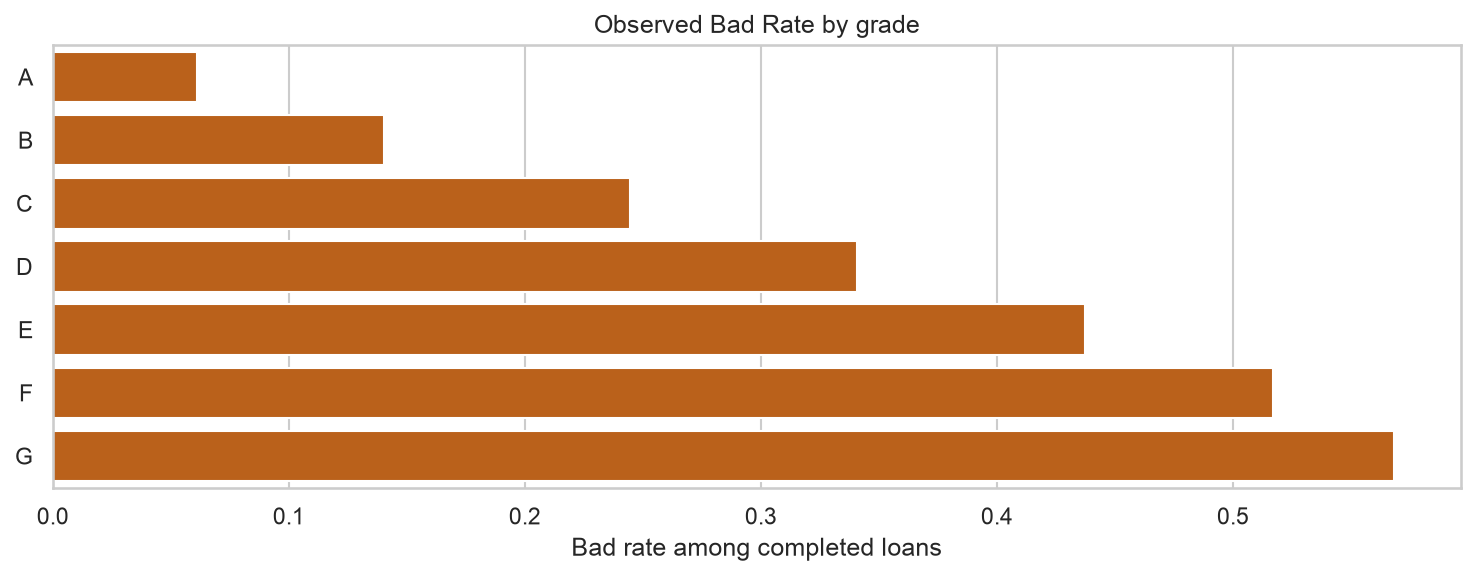
\includegraphics[width=0.74\linewidth]{../../EDA/accepted_eda_outputs/plots/observed_bad_rate_by_grade.png}
\caption{Observed bad rate by LendingClub grade in accepted-loan EDA.}
\label{fig:eda-grade}
\end{figure}

Continuous borrower and loan variables also behave consistently with credit-risk intuition. Higher debt-to-income ratio, higher revolving utilization, larger requested amount, longer term, and recent account-opening activity are associated with elevated risk. Higher FICO and higher income are associated with lower modeled risk, although income is skewed and must be interpreted carefully because high-income outliers can distort averages.

Several derived features make the raw LendingClub fields usable:
\[
\text{fico\_mean}=\frac{\text{fico\_range\_low}+\text{fico\_range\_high}}{2}
\]
\[
\text{credit\_history\_years}=\frac{\text{issue\_date}-\text{earliest\_credit\_line}}{365.25}.
\]
These transformations retain source traceability while producing numeric features appropriate for modeling.

Missingness was treated as a modeling signal only when defensible. Joint-applicant variables are structurally missing for individual applications, public-record recency variables are often missing because no record exists, and employment length has modest missingness that may itself be weakly predictive. The cleaning plan therefore distinguishes ordinary imputation from structural missingness and recommends missingness indicators or model-native missing handling where appropriate.

Temporal analysis motivated chronological validation. LendingClub volume, grade mix, interest rates, and observed bad rates vary across issue years. A random split would mix vintages and could make future-period performance appear better than it is. The final split therefore trains on older loans, validates on the next period, and evaluates once on the newest holdout.

\section{Methods}
Let $y\in\{0,1\}$ indicate whether a completed accepted loan charged off. Each model estimates a score $\hat{p}(x)=P(y=1\mid x)$. Logistic Regression models the log-odds as a linear function of cleaned and encoded predictors, using the sigmoid transformation to produce probabilities. Its binary cross-entropy objective penalizes confident wrong predictions and provides a transparent baseline for comparison.

Tree and gradient-boosting models handle nonlinear tabular structure. Random Forest averages many decorrelated decision trees to reduce variance. HistGradientBoosting, LightGBM, XGBoost, and CatBoost build additive ensembles of trees, where each new tree improves residual errors from earlier trees. These methods are suitable for LendingClub-style data because feature interactions are expected: for example, the risk meaning of loan amount depends on income, term, interest rate, and credit history.

The project evaluates discrimination and minority-class detection rather than accuracy. Precision is the share of predicted-risky loans that actually charged off; recall is the share of actual charge-offs captured. Their harmonic mean is
\[
F_1=2\cdot\frac{\text{precision}\cdot\text{recall}}{\text{precision}+\text{recall}}.
\]
ROC-AUC summarizes pairwise ranking over all thresholds, while PR-AUC focuses on the charged-off minority class and is more informative when the default base rate is low.

Calibration and thresholding translate rankings into decisions. Platt sigmoid calibration was used before probability-based policy analysis. A simple best-F1 threshold maximizes a technical metric but can over-review applicants, so the business policy uses an expected-value rule,
\[
\text{EV}=TP\cdot L_{\text{saved}}-FP\cdot C_{\text{opportunity}},
\]
with a maximum review/rejection share. In the example policy, catching a default saves \$10,000, rejecting a good borrower costs \$1,500, and the break-even default probability is 13.04\%.

SHAP is used after model selection to explain the preferred XGBoost model. The SHAP workflow computes global mean absolute importance, dependence plots, and borrower-level examples on a reproducible 5,000-row validation sample with seed 42, then checks stability on the test period. These outputs explain model behavior; they are not compliance-approved adverse-action reasons.

\section{Experimental Setup}
The final modeling frame contains 1,345,310 completed accepted loans. The chronological split is: train, 962,641 rows with 18.83\% bad rate and issue dates from 2007-06-01 to 2016-04-01; validation, 186,920 rows with 24.68\% bad rate and issue dates from 2016-05-01 to 2017-02-01; and test, 195,749 rows with 21.03\% bad rate and issue dates from 2017-03-01 to 2018-12-01.

Preprocessing starts from leakage-screened fields, creates the 38-feature starter set, encodes categorical variables, handles missing values consistently across splits, and exports baseline and no-grade/subgrade feature matrices. The project includes a PR-AUC-optimized advanced candidate search for LightGBM, XGBoost, and CatBoost, with candidates ranked by validation PR-AUC. For classification operating-point tables, thresholds are then chosen on validation F1 for the charged-off class so precision, recall, and F1 can be reported at a concrete cutoff. The test set is held out for final comparison, ablation confirmation, calibration review, and policy reporting.

The model notebooks are organized under \texttt{Modeling/}: preprocessing notebook 0, family notebooks 1--6 for Logistic Regression through CatBoost, advanced pipeline notebook 7, grade/interest ablation notebook 8, and final comparison notebook 9. TODO: add exact public notebook cell anchors after the repository is published.

Reproducibility artifacts include CSV outputs for split summaries, candidate metrics, selected metrics, ablations, calibration, economic policy, and SHAP interpretation. The environment is documented in \texttt{environment.yml} and \texttt{requirements.lock.txt}; SHAP interpretation requires \texttt{shap==0.51.0} because earlier versions had compatibility issues with the XGBoost serialization used here.

\section{Results}
Table~\ref{tab:model-results} compares the main model families at the best-validation-F1 operating point, while Figure~\ref{fig:prauc} summarizes PR-AUC ranking performance. The project also ran a PR-AUC-optimized advanced experiment: the top validation PR-AUC candidate was an XGBoost model with grade/subgrade (validation PR-AUC 0.4254), close to the F1-selected LightGBM baseline (validation PR-AUC 0.4248). Gradient boosting methods therefore perform similarly, and the final preferred neutral XGBoost no-grade/subgrade model is chosen for its governance and interpretation tradeoff rather than because it maximizes a single metric.

\begin{table}[h]
\centering
\small
\caption{Model comparison at selected validation threshold.}
\label{tab:model-results}
\begin{tabular}{lrrrrrrrrrr}
\toprule
Model & Val ROC & Val PR & Val P & Val R & Val F1 & Test ROC & Test PR & Test P & Test R & Test F1\\
\midrule
Logistic Regression & .695 & .412 & .355 & .698 & .471 & .700 & .362 & .311 & .709 & .432\\
Random Forest & .695 & .415 & .360 & .672 & .468 & .704 & .371 & .321 & .674 & .435\\
HistGradientBoosting & .701 & .424 & .359 & .697 & .474 & .708 & .377 & .320 & .693 & .438\\
LightGBM & .703 & .425 & .354 & .723 & .475 & .711 & .381 & .316 & .718 & .439\\
XGBoost & .702 & .425 & .358 & .701 & .474 & .710 & .380 & .319 & .701 & .438\\
CatBoost & .699 & .421 & .359 & .689 & .472 & .706 & .374 & .317 & .697 & .436\\
Preferred neutral XGB & .702 & .426 & .361 & .696 & .475 & .710 & .381 & .330 & .660 & .440\\
\bottomrule
\end{tabular}
\end{table}

\begin{figure}[h]
\centering
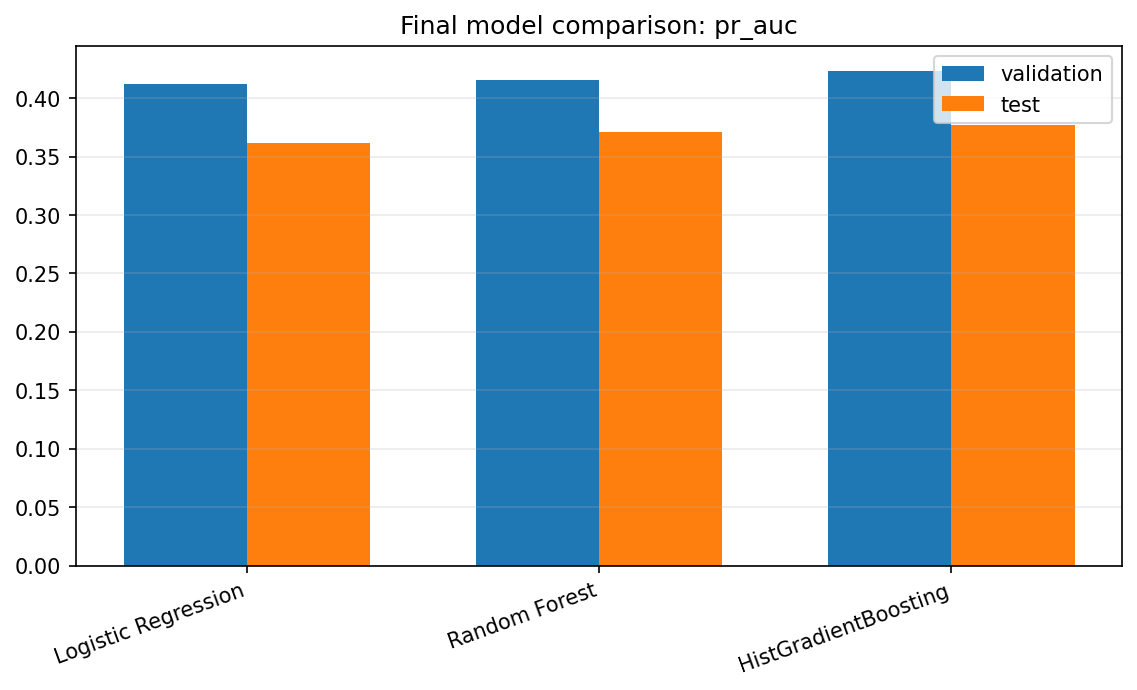
\includegraphics[width=0.72\linewidth]{../../Modeling/modeling_outputs/final_comparison/plots/final_model_pr_auc_comparison.png}
\caption{Final model PR-AUC comparison, used to evaluate minority-class ranking quality alongside F1-based operating thresholds.}
\label{fig:prauc}
\end{figure}

The preferred model is the neutral no-grade/subgrade XGBoost variant that retains \texttt{int\_rate\_clean}. On validation it reaches ROC-AUC 0.702, PR-AUC 0.426, precision 0.361, recall 0.696, and F1 0.475 for charged-off loans. On test it reaches ROC-AUC 0.710, PR-AUC 0.381, precision 0.330, recall 0.660, and F1 0.440. Its mean raw predicted probability on test is 0.197, close to the actual test bad rate of 0.210, which is preferable to earlier class-weighted models with inflated probabilities.

The ablation in Table~\ref{tab:ablation} shows that explicit grade/subgrade and interest rate carry overlapping information. Removing grade/subgrade while keeping \texttt{int\_rate\_clean} slightly improves validation PR-AUC and test top-20\% bad rate compared with keeping both, while avoiding direct dependence on LendingClub's discrete risk buckets. Removing both grade/subgrade and interest rate causes the clearest degradation.

\begin{table}[h]
\centering
\small
\caption{Grade/subgrade and interest-rate ablation.}
\label{tab:ablation}
\begin{tabular}{lrrrr}
\toprule
Feature policy & Val PR & Test PR & Test ROC & Test top-20\% bad\\
\midrule
Grade/subgrade + interest & .426323 & .380704 & .710495 & 39.98\%\\
No grade/subgrade + interest & .426423 & .380806 & .710201 & 40.09\%\\
Grade/subgrade, no interest & .426470 & .381304 & .710762 & 39.98\%\\
No grade/subgrade, no interest & .422215 & .375358 & .703070 & 39.64\%\\
\bottomrule
\end{tabular}
\end{table}

The best-F1 operating point is not a good business policy by itself. For the preferred model, the best-F1 threshold flags 42.07\% of test loans as risky. That catches many charge-offs, but the review or rejection volume is operationally and fairness-sensitive. A capped economic policy is more realistic because it imposes a maximum action share and evaluates the tradeoff between caught defaults and rejected good borrowers.

\begin{table}[h]
\centering
\small
\caption{Operating-policy comparison.}
\label{tab:policy}
\begin{tabular}{lrrrrr}
\toprule
Policy & Action share & Default capture & Bad rate in action group & Approved bad rate & Est. value\\
\midrule
Best-F1 threshold & 42.07\% & 66.02\% & 33.01\% & 12.3\% & $\approx$\$189.0M\\
Capped economic policy & 19.47\% & 37.43\% & 40.44\% & 16.34\% & \$120.0M\\
\bottomrule
\end{tabular}
\end{table}

SHAP confirms that the selected model is using plausible credit-risk signals. The top mean absolute SHAP drivers are \texttt{int\_rate\_clean}, \texttt{term\_months}, \texttt{acc\_open\_past\_24mths}, \texttt{dti}, \texttt{fico\_mean}, \texttt{annual\_inc}, and \texttt{loan\_amnt}. Validation-versus-test SHAP rank stability has Spearman correlation 0.9987, indicating that the main explanation ranking is not merely a validation-period artifact.

\begin{figure}[h]
\centering
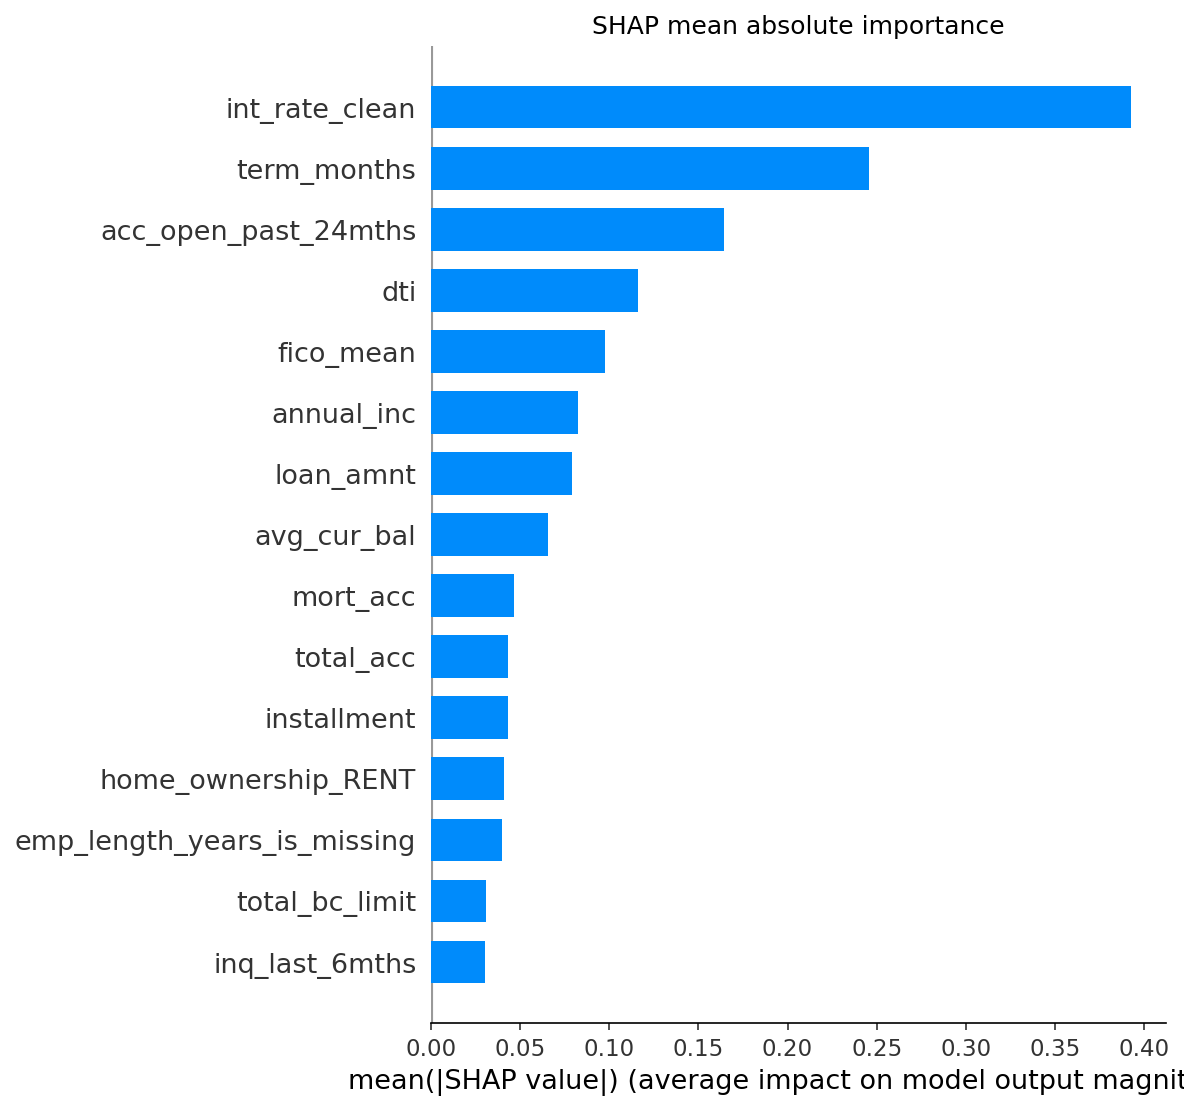
\includegraphics[width=0.72\linewidth]{../../Interpretation_SHAP/shap_outputs/plots/shap_mean_abs_bar.png}
\caption{Global SHAP mean absolute importance for the preferred model.}
\label{fig:shap}
\end{figure}

The project could likely improve raw predictive performance with larger ensembles, borrower text fields, broader credit-bureau variables, or more aggressive hyperparameter searches. Those options were not the main recommendation because the course project also values defensible data handling, leakage control, and explainability. A stronger but less governed model would be less aligned with the credit-risk interpretation and future RAG explanation goal.

\section{Analysis and Discussion}
The algorithms work because consumer-credit risk is nonlinear and interaction-heavy. Interest rate, term, installment burden, DTI, income, FICO, recent account openings, and loan amount do not act independently. Tree ensembles can partition these interactions without requiring every cross-feature relationship to be manually specified.

The selected feature policy illustrates a governance tradeoff. LendingClub grade and subgrade are powerful, but they are also summaries of LendingClub's prior underwriting and pricing process. Retaining the continuous interest-rate signal while removing discrete grade buckets keeps much of the risk information but reduces dependence on an opaque categorical prior decision. This does not eliminate all governance concerns, because interest rate itself reflects pricing policy, but it is more parsimonious and easier to analyze.

Temporal drift is visible in the split bad rates and in the need for future-period testing. The validation bad rate is 24.68\%, while the test bad rate is 21.03\%. This difference reinforces why calibration, monitoring, and threshold review matter. A model trained on older vintages can rank risk in a later period, but policy thresholds should not be assumed permanent.

The lessons generalize to similar consumer-credit datasets where outcomes arrive after origination and many fields are updated after the decision. Leakage audits, time-based validation, calibrated probabilities, PR-AUC, top-risk precision, and capped decision policies are broadly useful. The exact model and threshold should not be transferred without local data, policy constraints, and fairness review.

Compared with published and Kaggle implementations, this project's novelty is not a new algorithm. Its contribution is a careful end-to-end workflow: accepted-loan target definition, rejected-applicant boundary, leakage-controlled features, chronological evaluation, grade/interest ablation, calibration, SHAP stability, and economic thresholding. The system should be treated as a research-grade risk-ranking and interpretation prototype rather than a production lending decision engine.

\section{Conclusion}
This project built a leakage-aware LendingClub accepted-loan default-risk modeling workflow from raw data through EDA, cleaning, preprocessing, model comparison, ablation, calibration, SHAP interpretation, and policy analysis. The preferred neutral XGBoost model predicts the probability of charge-off for accepted loans and achieves stable ranking performance on a future-period test set.

For a company evaluating a similar internal prototype, the recommended approach is not the unconstrained best-F1 threshold. The better research recommendation is the no-grade/subgrade neutral XGBoost model with calibrated probabilities and a capped review or rejection policy, because it balances risk concentration, operational volume, and interpretability more clearly than raw F1 optimization.

Future work should complete the RAG explanation layer only after reason-code governance, compliance review, fairness analysis, external validation, monitoring design, and deployment documentation. The next phase should map SHAP-supported technical drivers to human-readable reason codes, retrieve regulatory context, generate constrained explanation drafts, and evaluate faithfulness without claiming legal adverse-action compliance.

\section{AI Prompts Used}
The repository contains a detailed EDA prompt in \texttt{Docs/Prompts/Prompt.md}. It asks an AI assistant to act as a principal data scientist and produce a rigorous LendingClub EDA covering business context, inventory, cleaning, target definition, missingness, distributions, time trends, leakage, accepted-versus-rejected comparisons, fairness, and modeling readiness. This LaTeX report was drafted from the final-report LaTeX drafting prompt in the report folder. TODO before submission: collect all coding, debugging, explanation, and research prompts used by the team and include the complete prompt text or a course-approved appendix.

\section{References}
\begin{thebibliography}{99}
\bibitem{kaggledata} Nathan George. ``All Lending Club loan data.'' Kaggle dataset. \url{https://www.kaggle.com/datasets/wordsforthewise/lending-club}.
\bibitem{kagglepython} Nathan George. ``EDA with Python.'' Kaggle notebook linked from the dataset page. \url{https://www.kaggle.com/wordsforthewise/eda-with-python}.
\bibitem{kaggler} Nathan George. ``EDA in R: arggghh.'' Kaggle notebook linked from the dataset page. \url{https://www.kaggle.com/wordsforthewise/eda-in-r-arggghh}.
\bibitem{kaggleoutliers} Mariia Gusarova. ``Detect and Remove the Outliers.'' Kaggle notebook. \url{https://www.kaggle.com/code/mariiagusarova/detect-and-remove-the-outliers}.
\bibitem{gupta2022} S. Gupta, R. Gulati, and A. Chakrabarty. ``Classification based credit risk analysis: The case of Lending Club.'' arXiv:2210.05136, 2022.
\bibitem{misheva2021} B. Hadji Misheva et al. ``Explainable AI in Credit Risk Management.'' arXiv:2103.00949, 2021.
\bibitem{demajo2020} L. M. Demajo, V. Vella, and A. Dingli. ``Explainable AI for Interpretable Credit Scoring.'' arXiv:2012.03749, 2020.
\bibitem{sanz2024} S. Sanz-Guerrero and J. Arroyo. ``Credit Risk Meets Large Language Models: Building a Risk Indicator from Loan Descriptions in P2P Lending.'' arXiv:2401.16458, 2024.
\bibitem{schwartz2025} M. Schwartz, Y. Wang, and S. Fang. ``Enhancing ML Models Interpretability for Credit Scoring.'' arXiv:2509.11389, 2025.
\bibitem{nortey2026} E. Nortey et al. ``An Optimised Greedy-Weighted Ensemble Framework for Financial Loan Default Prediction.'' arXiv:2603.18927, 2026.
\bibitem{solozobov2026} A. Solozobov. ``Label-Free Detection of Governance Evidence Degradation in Risk Decision Systems.'' arXiv:2604.17836, 2026.
\end{thebibliography}

\appendix
\section{Appendix}
Public GitHub repository URL: TODO if not public yet. If the repository cannot be made public, submit the project as a zip file on Canvas according to the assignment instructions.

Setup summary: install the Python environment from the project environment or lock file; place the Kaggle accepted and rejected LendingClub files under \texttt{Data/archive/}; run EDA, cleaning, preprocessing, model notebooks, final comparison, and SHAP interpretation in order. The main artifact folders are the EDA, cleaning, preprocessing, modeling-output, and SHAP-output directories.

Notebook inventory: accepted-loan EDA, accepted-loan cleaning, preprocessing notebook 0, model notebooks 1--9 under \texttt{Modeling/}, and SHAP interpretation notebook 1. Extra plots and CSV tables are stored beside each notebook output folder.

\section{Statement of Contributions}
Linda Perez Penaranda: project lead, credit-risk framing, EDA, cleaning, modeling, policy analysis, reproducibility, and report integration. Yashaswi Aryan: collaborator on model/retrieval workflow and project development. Siddharth Agarwal: collaborator on model/retrieval workflow and project development. TODO before submission: verify this contribution statement with all team members.

\end{document}
